\documentclass[a4paper, 12pt]{article}

\usepackage[english,russian]{babel}
\usepackage[T2A]{fontenc}
\usepackage[utf8]{inputenc}
\usepackage{geometry}
\usepackage{enumitem}
\usepackage{setspace}
\usepackage{amssymb}
\usepackage{graphicx}
\usepackage{wrapfig}
\usepackage{float}
\usepackage{amsmath}
\usepackage{textcomp}
\usepackage{dsfont}

\geometry{top=5mm, left=1cm}
%\setlength{\parindent}{0}
\renewcommand{\arraystretch}{1.2}
\linespread{1}

\begin{document}
    \begin{center}
        \textbf{Сферическая геометрия тест №3}\\
        Прямые, полюсы, поляры
    \end{center}

    \begin{center}
        \textbf{№ 1}
    \end{center}

    Угол между двумя секущими плоскостями равен $\alpha$.
    Чему равен угол между двумя прямыми,
    каждая из которых соединяет полюсы соответсвующий плоскостей?

    \textbf{Решение}\\

    \begin{center}
        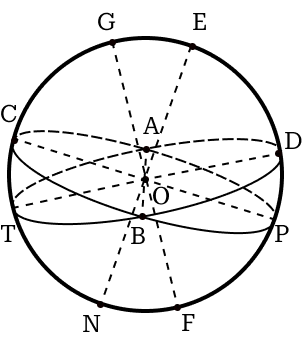
\includegraphics[width=0.2\textwidth]{images/img1} \quad
        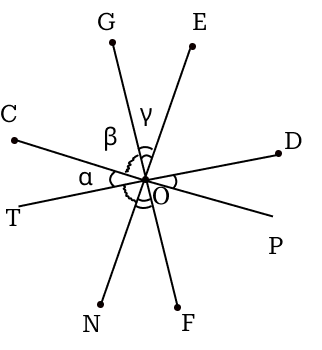
\includegraphics[width=0.2\textwidth]{images/img2}\\
    \end{center}

    1) Так как секущие прямые имеют общую точку, то они пересекаются по прямой $AB$, что следует из аксиом стереометрии.

    2) Восстановим перпендикуляр $OC\bot AB$ в плоскости $(BOC)$ и перпендикуляр $OD \bot AB$ в плоскости $BOD$.
    Проведем прямые, соединяющие полюсы $GF$ и $EN$, так как прямая $AB$ лежит в плоскостях сечений,
    то $CF \bot AB$ и $EN \bot AB$.

    3) $OC \bot AB$, $OD \bot AB$, $GF \bot AB$, $EN \bot AB$,
    тогда эти прямые ($OC, OD, GF, EN$) лежат в плоскости $(COE)$, перпендикулярной прямой $AB$.

    4) Вынесем планиметрический чертеж, на котором $\angle COT = \alpha$ - линейный угол двугранного угла $CABT$,
    который равен углу между секущими плоскостями.
    Так как $GF \bot (TOA)$, то $GF \bot TD \subset (TOA)$ и так как $EN \bot (COP)$, то $EN \bot CP \subset (COP)$.
    Получаем, что $\beta = 90^\circ - \alpha = \angle COT$

    5) Таким образом:
    \[
        2\beta + \alpha + \gamma = 180^{\circ}
    \]
    \[
        180^{\circ} - 2\alpha + \alpha + \gamma = 180 ^{\circ}
    \]
    \[ \alpha = \gamma \]

    Ответ: $\alpha$

    \begin{center}
        \textbf{№ 2}
    \end{center}

    Чему равна площадь четырехугольника, образованного двумя полисами и диаметрально противоположными точками поляры,
    если радиус сферы $R$.

    \textbf{Решение}\\

    \begin{center}
        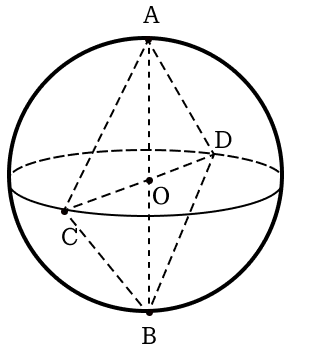
\includegraphics[width=0.2\textwidth]{images/img3}\\
    \end{center}

    1) $CO = DO = AO = BO = R$

    2)
    \[
        S_{ABCD} = S_{\triangle AOC} + S_{\triangle BOC} + S_{\triangle BOD} + S_{\triangle DOA} = 4 S_{\triangle BOC} = 4 * \frac{AO * CO}{2} = 2R^2
    \]

    Ответ: $2R^2$





\end{document}
